\section{Raven Tutorial}
\label{sec:ravenTutorial}

\subsection{Overview}
\label{sub:overview}
RAVEN is a multi-purpose software framework designed to perform parametric and stochastic analysis based on the
response of complex system codes. The initial development was designed to provide dynamic probabilistic risk
analysis capabilities (DPRA) to the thermal-hydraulic code RELAP-7, currently under development at Idaho National
Laboratory (INL).
Now, RAVEN is not only a framework to perform DPRA but it is a multi-purpose stochastic and uncertainty 
quantification platform, capable of communicating with any system code through the provided  Application
Programming Interfaces (APIs). These APIs allow RAVEN to interact with any code as long as all the parameters
that need to be perturbed are accessible through input files or via  \texttt{Python} interfaces. RAVEN is capable
of investigating the system response as well as the input space using sampling schemes, such as Monte Carlo, Grid,
Latin Hyper Cube. However, RAVEN strength is the set of system feature discovery capabilities.

\subsection{Example Model: Analytic Bateman}\label{sec:analyticalbateman}
This section is intended for the new users to familiarize them with how to perform their studies through RAVEN.
A simple example, conventionally called \textbf{AnalyticBateman}, has been developed. It solves a system of
ordinary differential equations (ODEs), of the form:

\begin{equation}
\begin{dcases}
\frac{\mathrm{d} \mathbf{X}}{\mathrm{d} t} = \mathbf{S}-\mathbf{L} \\
 \mathbf{X}(t=0)= \mathbf{X_{0}}
\end{dcases}
\end{equation}
   where:
  \begin{itemize}
     \item $\mathbf{X_{0}}$, initial conditions
     \item $\mathbf{S}$, source terms
     \item $\mathbf{L}$, loss terms
   \end{itemize}

For example, this  code is able to solve a system of two ODEs as follows:
\begin{equation}
  \begin{dcases}
    \frac{\mathrm{d} x_{1}}{\mathrm{d} t} = \phi (t)\times \sigma_{x_{1}}-\lambda_{x_{1}}\times x_{1}(t) \\
    \frac{\mathrm{d} x_{2}}{\mathrm{d} t} = \phi (t)\times \sigma_{x_{2}}-\lambda_{x_{2}} \times x_{2}(t) + x_{1}(t)\times\lambda_{x_{1}} \\
    x_{1}(t=0)= x_{1}^{0} \\
    x_{2}(t=0)= 0.0
  \end{dcases}
\end{equation}

The input of the \textbf{AnalyticBateman} code is in XML format.
For example, the following is the reference input for a system of 4 Ordinary Differential Equations (ODEs)
that is going to be used for as an example in this guide. All the files required for this system are  located at
``\textit{raven/tests/framework/user\textunderscore guide/physicalCode}''. 

\xmlExample{framework/user_guide/physicalCode/analyticalbateman/Input.xml}{AnalyticalBateman}
The code outputs the time evolution of the 4 variables ($A,B,C,D$) in a CSV file, producing the following output:
\begin{table}[ht]
\centering
\caption{Reference case sample results.}
\label{referenceResults}
\begin{tabular}{lllll}
\textbf{time} & \textbf{A}     & \textbf{C}     & \textbf{B}    & \textbf{D}     \\
0                  & 1.0                       & 1.0                       & 1.0                     & 1.0           \\
2880000.0   & 0.983434738239 & 0.977851848235 & 1.01011506729 & 1.01013172275 \\
5760000.0   & 0.967143884376 & 0.956202457404 & 1.01936231677 & 1.02036100400   \\
8640000.0   & 0.951122892771 & 0.935040450532 & 1.02777406275 & 1.03067925987 \\
10368000.0 & 0.941637968936 & 0.922572556179 & 1.03243314106 & 1.03690947068 \\
12096000.0 & 0.932247632016 & 0.910273757371 & 1.03680933440 & 1.04316700086 \\
13824000.0 & 0.922950938758 & 0.898141730426 & 1.04090912054 & 1.04945015916 \\
15552000.0 & 0.913746955315 & 0.886174183908 & 1.04473885709 & 1.05575729317 \\
17280000.0 & 0.904634757153 & 0.874368858183 & 1.04830478357 & 1.06208678854 \\
20736000.0 & 0.886682064542 & 0.851235986899 & 1.05466958557 & 1.07480659230  \\
24192000.0 & 0.869085647400 & 0.828725658721 & 1.06005115510 & 1.08759739100   \\
27648000.0 & 0.851838435355 & 0.806820896763 & 1.06449535534 & 1.10044757060  \\
31104000.0 & 0.834933498348 & 0.785505191756 & 1.06804634347 & 1.11334606143 \\
34560000.0 & 0.818364043850 & 0.764762489077 & 1.07074662835 & 1.12628231792
\end{tabular}
\end{table}

\pagebreak
\subsection{Build RAVEN input: \xmlNode{SingleRun}}
\label{sub:singleRun}
In this section, we will show the user how to use RAVEN to run a single instance of a driven code, and
printing some variables. 
We will start to build a very simple RAVEN input, and this input file can be found at 
``\textit{raven/tests/framework/user\textunderscore guide/ravenTutorial/singleRun.xml}''. 
From this process, we hope the user can get a better idea about
RAVEN entities and learn how to build their own RAVEN inputs for their applications.
In order to accomplish these tasks, the following procedures are needed:
\begin{enumerate}
   \item \textbf{Set up the running environment}: \xmlNode{RunInfo}
     \\The \textbf{RunInfo} entity is an information container which describes how the overall computation should
      be performed. This Entity accepts several input settings that define how to drive the calculation and set up,
      when needed, particular settings for the machine the code needs to run on (queue system, if not Portable
      Batch System-PBS, etc.). For the simple case, the \textbf{RunInfo} will look like:
      \xmlExample{framework/user_guide/ravenTutorial/singleRun.xml}{RunInfo}
      In this specific case, only one step named \xmlString{single} is going to be sequentially run using a single
      processor as defined by \xmlNode{BatchSize}. All the output files and temporary files will be dumped in the
      folder \xmlString{singleRunAnalysis}.

   \item \textbf{Provide the required files}: \xmlNode{Files}
     \\ The \textbf{Files} entity  defines any files that might be needed within the RAVEN run. This could include
     inputs to the Model, pickled ROM files, or Comma Separated Value (CSV) files for post-processors, to name a few.
     Each entry in the \xmlNode{Files} block is a tag with the file type. Files given through the input XML at this
     point are all \xmlNode{Input} type. Each \xmlNode{Input} node has a required attributes \xmlAttr{name}. It does
     not need to be the actual filename, and it is the name by which RAVEN will use to identify the specific file. Other
     optional attributes are not directly used by RAVEN, and they are mainly used by the \textbf{CodeInterface}. More
     detailed information can be found in the user manual ~\cite{RAVENuserManual}. For the simple case, the \textbf{Files}
     will look like:
     \xmlExample{framework/user_guide/ravenTutorial/singleRun.xml}{Files}
     This RAVEN input file shows that the user will provide a file that is located at ``\textit{../commonFiles/referenceInput.xml}''
     with reference name \xmlString{referenceInput.xml}. This file will be available for use via other RAVEN input blocks or entities.
     In this case, a relative path to the working directory specified via \xmlNode{WorkingDir} under node \xmlNode{RunInfo}
     is used.

   \item \textbf{Link between RAVEN and driven code}: \xmlNode{Models}
     \\ The \textbf{Models} entity represents the projection from the input to the output space. In other words,
     the Model entity can be seen as a transfer function between the input and output space. Currently, RAVEN
     defines the following sub-entities:
     \begin{itemize}
       \item \textit{Code}, represents the driven code, through external code interfaces (see~\cite{RAVENuserManual})
       \item  \textit{ExternalModel}, represents a physical or mathematical model that is directly implemented by
         the user in a Python module
       \item \textit{ROM}, represents the Reduced Order Model, interfaced with several algorithms
       \item \textit{PostProcessor}, is used to perform action on data, such as computation of statistical moments,
         correlation matrices, etc.
     \end{itemize}
     For simplicity, only \textit{Code} is used here for the demonstration, and the input block looks like:
     \xmlExample{framework/user_guide/ravenTutorial/singleRun.xml}{Models}
     As shown in the \xmlNode{Models} block, the subnodes defined for \xmlNode{Code} is equivalent to:
     \begin{lstlisting}[language=bash]
     python ../physicalCode/analyticalbateman/AnalyticalDplMain.py
     \end{lstlisting}
     with the requirement of extensions of input and output files, as defined via \xmlNode{clargs}, to be 
     \xmlString{.xml} and \xmlString{.csv}, respectively. In this case, the \textbf{GenericCode} interface is employed.
     This interface is meant to handle a wide variety of generic codes that take straightforward input files and produce
     CSV files. \nb If a code contains cross-dependent data, the generic interface is not applicable. For more detailed
     information, the user can refer to section \textbf{Existing Interface} of the user manual ~\cite{RAVENuserManual}.

   \item \textbf{Container of input and output data}: \xmlNode{DataObjects}
     \\The \textbf{DataObjects} system is a container of data objects of various types that can be constructed
     during the execution of desired calculation flow. These data objects can be used as input or output for a
     particular \textbf{Model} Entity. Currently RAVEN supports the following data types, each with a particular
     conceptual meaning:
     \begin{itemize}
        \item \textit{PointSet} is a collection of individual objects, each describing the state of the system at
                                a certain point (e.g. in time). It can be considered a mapping between multiple
                                            sets of parameters in the input space and the resulting sets of outcomes in the output space
                                            at a particular point (e.g., in time).
        \item \textit{HistorySet} is a collection of individual objects, each describing the temporal evolution of the
                                  state of the system within a certain input domain. It can be considered a mapping between
                                               multiple sets of parameters in the input space and the resulting sets of temporal evolution
                                               in the output space.
     \end{itemize}
     The DataObjects represent the preferred way to transfer the information coming from a Model (e.g., the
     driven code) to all the other RAVEN systems (e.g., Out-Stream system, Reduced Order Modeling component, etc.).
     For the simple case, the \xmlNode{DataObjects} block of RAVEN input is:
     \xmlExample{framework/user_guide/ravenTutorial/singleRun.xml}{DataObjects}
     \xmlNode{HistorySet} with a user-defined identifier (e.g. ``history'') is used to collect the mass evolutions
     of four given isotopes, i.e. A, B, C, D. \xmlNode{Input} node is used to list the input parametes to which
     this data is connected. If there is no input data associated with this node, the \xmlString{InputPlaceHolder}
     can be used. \xmlNode{Output} is used to list the output parameters to which this data is connected. Similarly,
     if there is no output data associated with this node, the \xmlString{OutputPlaceHolder} can be used. This is
     mainly because both \xmlNode{Input} and \xmlNode{Output} nodes are required for all types of \textbf{DataObjects}.

    \item \textbf{Print and plot input and output data}: \xmlNode{OutStreams}
      \\ The OutStreams node is the entity used for data exporting and dumping. The OutStreams support
      2 actions:
      \begin{itemize}
       \item \textit{Print}. This Out-Stream is able to print out (in a Comma Separated Value format) all the information
         contained in:
         \begin{itemize}
          \item DataObjects
          \item Reduced Order Models.
         \end{itemize}
       \item \textit{Plot}. This Out-Stream is able to plot 2-Dimensional, 3-Dimensional, 4-Dimensional (using color
       mapping) and 5-Dimensional (using marker size). Several types of plot are available, such as scatter, line, surfaces,
       histograms, pseudo-colors, contours, etc.
      \end{itemize}
      In this case, a simple \xmlNode{OutStreams} is used to output the mass evolutions of all four model variables
      into a CSV file with the name prefix ``print\textunderscore history''.
      \xmlExample{framework/user_guide/ravenTutorial/singleRun.xml}{OutStreams}

    \item \textbf{Control of executions}: \xmlNode{Steps}
      \\The \textbf{Steps} entity is used to create a peculiar analysis flow via combining together different RAVEN
      entities. It is the location where all the defined entities get finally linked in order to perform a combined
      action on a certain \textit{Model}. In order to perform this linking, each entity defined in the Step needs to
      ``play'' a role:
      \begin{itemize}
        \item \textit{Input} represents the input of the step. The allowable input objects depend on the type
          of \textit{Model} in this step.
        \item \textit{Model} represents a physical or mathematical system or behavior. The object used in this role
          defines the allowable types of inputs and outputs usable in this step.
        \item \textit{Output} defines where to collect the results of an action performed by the \textit{Model}. It
          is generally one of the following types: \textbf{DataObjects}, \textbf{Databases}, or \textbf{OutStreams}.
        \item \textit{Sampler} defines the sampling strategy to be used to probe the model. \nb When a sampling
          strategy is employed, the "variables" defined in the \xmlNode{variable} blocks are going to be directly
          placed in the output objects of type \textbf{DataObjects} and \textbf{Databases}.
        \item \textit{Function} is an extremely importance role. It introduces the capability to perform pre or post
          processing of model inputs and outputs. Its specific behavior depends on the step is using it.
        \item \textit{ROM} defines an acceleration reduced order model to use for a step.
        \item \textit{SolutionExport}, represents the container of the eventual output of a step. It is the entity
          that is used to export the solution of a \textit{Sampler} or post-processors.
      \end{itemize}
      Currently, RAVEN supports the following types of \textit{\xmlNode{Steps}}:
      \begin{itemize}
        \item \textit{SingleRun}, perform a single run of a model
        \item \textit{MultiRun}, perform multiple runs of a model
        \item \textit{RomTrainer}, perform the training of a Reduced Order Model (ROM)
        \item \textit{PostProcess}, post-process data or manipulate RAVEN entities
        \item \textit{IOStep}, step aimed to perform multiple actions:
        \begin{itemize}
          \item construct/update a Database from a DataObjects and vice-versa
          \item construct/update a Database or a DataObjects object from CSV files
          \item stream the content of a Database or a DataObjects out through an OutStream
          \item store/retrieve a ROM to/from an external File using Pickle module of Python
        \end{itemize}
      \end{itemize}
      For this example, the \xmlNode{SingleRun} is used to assemble a calculation flow, i.e. perform a single action
      of a model.
      \xmlExample{framework/user_guide/ravenTutorial/singleRun.xml}{Steps}
      The code ``testModel'' will be executed once, and the outputs will be collected into a \xmlString{DataObjects}
      of type \textbf{HistorySet}. In addition, \xmlString{OutStreams} is used to print the output data into a CSV file.
\end{enumerate}

The core of the RAVEN calculation flow is the \textbf{Steps} system. The \textbf{Steps} is in charge of assembling
different entities in RAVEN in order to perform a task defined by the kind of step being used
(see Figure.~\ref{fig:ExampleStepEntity}).

\begin{figure}[h!]
  \includegraphics[scale=1]{pics/ExampleStepEntity.png}
  \caption{Example of the Steps \textbf{Entity}  and its connection in the input file.}
  \label{fig:ExampleStepEntity}
\end{figure}

%%%%%%%%%%%%%%%%%%%%%%%%%%%%%%%%%%%%%%%%%%%%%%%%%%%%%%%%%%%%%%%%%
%%%%%%%%%%%%%%%%%%%%%%%%%%%%%%%%%%%%%%%%%%%%%%%%%%%%%%%%%%%%%%%%%
\subsection{Build RAVEN Input: \xmlNode{IOStep}}
The \xmlNode{IOStep} acts as a "transfer network" among different RAVEN storing or streaming objects. The number
of \xmlNode{Input} and \xmlNode{Output} is unlimited. This \xmlNode{IOStep} assumes one-to-one mapping, i.e. the first
\xmlNode{Input} is going to be used for the first \xmlNode{Output}, etc. \nb If the \xmlNode{Output} nodes are class
\xmlString{OutStreams}, the user does not need to follow this assumption, since \textbf{OutStreams} objects are already
linked to \textbf{DataObjects} in the relative RAVEN input block.
The \textbf{IOStep} can be used to:
\begin{itemize}
  \item construct/update a \textit{Database} from a \textit{DataObjects} object, and vice versa;
  \item construct/update a \textit{DataObject} from a \textit{CSV} file contained in a directory;
  \item construct/update a \textit{Database} or a \textit{DataObjects} object from
    \textit{CSV} files contained in a directory;
  \item stream the content of a \textit{Database} or a \textit{DataObjects} out through an \textbf{OutStream} object;
  \item store/retrieve a \textit{ROM} to/from an external \textit{File} using Pickle module of Python.
\end{itemize}
The last function can be used to create and store mathematical model of fast solution trained to predict a
response of interest of a physical system. This model can be recovered in other simulations or used to evaluate
the response of a physical system in a Python program by the implementing of the Pickle module.

%%%%%%%%%%%%%%%%%%%%%%%%%%%%%%%%%%%%%%%%%%%%%%%%%%%%%%%%%%%%%%%%%
\subsubsection{Perform input/output operations}
In this case, we will use \xmlNode{IOStep} to stream the output data from the \textit{DataObjects} out through the
\textit{OutStreams}. The \xmlNode{IOStep} block is shown as follows:
\xmlExample{framework/user_guide/ravenTutorial/singleRunPlotAndPrint.xml}{Steps}
As shown in the \xmlNode{IOStep}, the input is a history set ``history'' that is previous generated by the \textbf{SingleRun}
step. The data stored in the ``history'' will be printed and plotted via the \textbf{OutStreams}.The data object
``history'' is defined as follows:
\xmlExample{framework/user_guide/ravenTutorial/singleRunPlotAndPrint.xml}{DataObjects}
\nb If a \textit{PointSet} data object is used to collect the temporal output data, only the data from the last time
step will be stored in this data object. As demonstrated in this case, the output csv file with name ``pointValues.csv''
generated through the \textbf{OutStreams} in \textbf{SingleRun} step only contains the data for the last time step.
This file can be found in the working directory specified by sub-node \xmlNode{WorkingDir} under node \xmlNode{RunInfo}.

As mentioned before, \textbf{OutStreams} can be used to plot the data stored in the data objects. The following
input block demonstrates the use of \textbf{OutStreams} for plotting.
\xmlExample{framework/user_guide/ravenTutorial/singleRunPlotAndPrint.xml}{OutStreams}
In this block, both the Out-Stream types are constructed:
\begin{itemize}
  \item \textit{Print}: named ``history'' connected with the \textit{DataObjects} \textbf{Entity} ``history'' (\xmlNode{source})
  When this object get used, all the information contained in the linked  \textit{DataObjects} are going
  to be dumped in CSV files (\xmlNode{type}).
  \item \textit{Plot}: a single \xmlNode{Plot} \textbf{Entity} is defined, containing the line plots of the 4 output variables
  ($A,B,C,D$) in the same figure. This object is going to generate a PNG file in the working directory.
\end{itemize}

%figure history
\begin{figure}[h!]
  \centering
  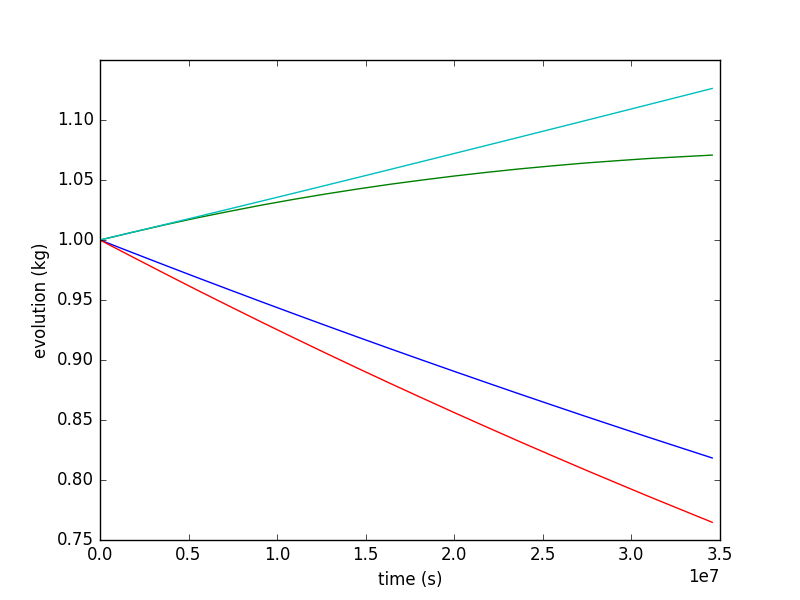
\includegraphics[scale=0.7]{../../tests/framework/user_guide/ravenTutorial/gold/singleRunPlot/1-historyPlot_line-line-line-line.png}
  \caption{Plot of the history for variables $A,B,C,D$.}
  \label{fig:historyPlotLine}
\end{figure}

For examples of the numerical data produced by the OutStreams \textit{Print}, see \texttt{history\_0.csv} in the directory
 \texttt{raven/tests/framework/user\_guide/ravenTutorial/ gold/singleRunPlot/}
 As previously mentioned, Figure~\ref{fig:historyPlotLine} reports the four plots (four variables) drawn in the same picture.

%%%%%%%%%%%%%%%%%%%%%%%%%%%%%%%%%%%%%%%%%%%%%%%%%%%%%%%%%%
%\FloatBarrier
\subsubsection{Sub-plot and selectively printing.}
This section shows how to use RAVEN to create sub-plots (multiple plots in the same figure) and
how to select only some variable from the \textit{DataObjects} in the \textit{Print} OutStream.
 \\ The goals of this Section are about learning how to:
 \begin{enumerate}
   \item Print out what contained in the DataObjects, selecting only few variables
   \item Generate sub-plots (multiple plots in the same figure) of the code results
\end{enumerate}

To accomplish these tasks, the \xmlNode{IOStep} needs to be modified as follows:
\xmlExample{framework/user_guide/ravenTutorial/singleRunSubPlotsAndSelectivePrint.xml}{Steps}
\nb as mentioned before, this \xmlNode{IOStep} does not need to follow the one-to-one mapping, since \textit{OutStreams}
are alreadly linked to the \textit{DataObjects}.
And the \textit{OutStreams} \textbf{Entity} in the input defined in the previous section needs to be modified as
follows:
\xmlExample{framework/user_guide/ravenTutorial/singleRunSubPlotsAndSelectivePrint.xml}{OutStreams}

\begin{enumerate}
   \item \textbf{\textit{Print}}:
   With respect to the \textit{Print} nodes defined in the previous section, it can
   be noticed that an additional node has been added: \xmlNode{what}. The \textit{Print} \textbf{Entity}
   ``pointValues'' is going to extract and dump only the variables that are part of the Output space
   ($A,B,C,D$ and not $InputPlaceHolder$).  The \textit{Print} \textbf{Entity} ``history'' is instead going to print
   the Output space variables $A$ and $D$.

   \item \textbf{\textit{Plot}}:
 Note that the  \textit{Plot} \textbf{Entity} does not differ much with respect to the one in
 previous section: 1) the additional sub-node \xmlNode{gridSpace}  has been added.
 This node is needed to define how the figure needs to be partitioned (discretization of the grid). In this case
 a 2 by 2 grid is requested. 2) in each \xmlNode{plot} the node \xmlNode{gridLocation} is placed in
 order to specify in which position the relative plot needs to be placed. For example, in the following grid
 location, the relative plot is going to be placed at the bottom-right corner.
 \begin{lstlisting}[style=XML,morekeywords={arg,extension,pauseAtEnd,overwrite}]
   <gridLocation>
      <x>1</x>
      <y>1</y>
   </gridLocation>
  \end{lstlisting}
\end{enumerate}

The printed data will dump to the CSV file \textit{history\_0.csv}, and Figure~\ref{fig:historySubPlotLine} reports the four plots (four variables) drawn in the same picture.

%figure history sublots
\begin{figure}[h!]
  \centering
  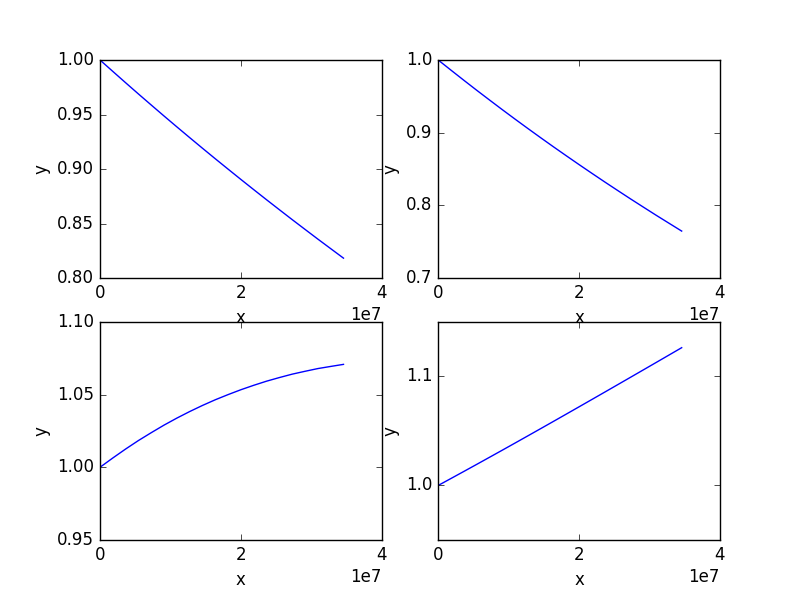
\includegraphics[scale=0.7]{../../tests/framework/user_guide/ravenTutorial/gold/subPlot/1-historyPlot_line-line-line-line.png}
  \caption{Subplot of the history for variables $A,B,C,D$.}
  \label{fig:historySubPlotLine}
\end{figure}


